\section{Modelo Neuronal}

Para la implementación de la red neuronal se utilizó la biblioteca de Tensor Flow, donde se utilizó una red neuronal simple con 2 neuronas de entrada, 5 neuronas en la capa oculta y 1 neurona en la capa de salida. La Figura \ref{fig:RedTF} muestra esta red.

\begin{figure}[H]
    \centering
    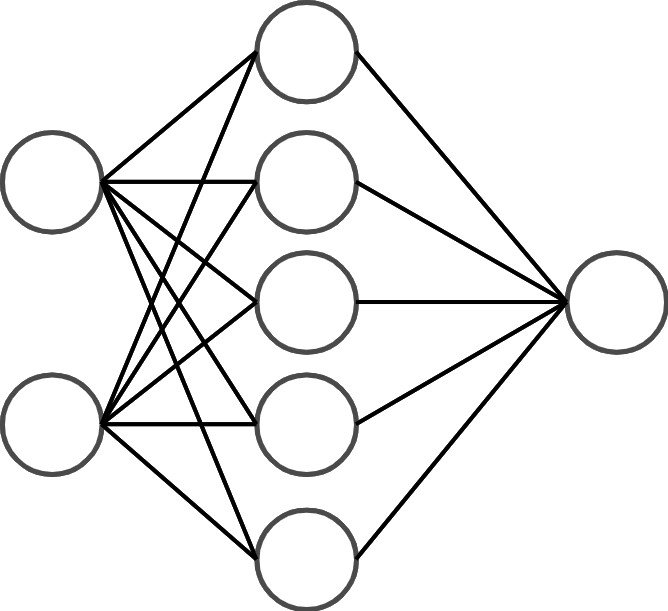
\includegraphics[width=0.5\textwidth]{Resultados/imgs/RedTF.png}
    \caption{Red neuronal implementada en Tensor Flow.}
    \label{fig:RedTF}
\end{figure}

Para la implementación con la biblioteca Tensor Flow se realizaron 1000 entrenamientos, ya que esta es la cantidad máxima permitida por los recursos del hardware utilizado, con los resultados de estos entrenamientos se obtuvo el valor mínimo el valor máximo y el promedio de todos los experimentos.

\subsection{Carril central}

La Tabla \ref{tab:resultadosTFCCentral} muestra los resultados para el carril central en kilómetros por hora, se nota que para estos experimentos el promedio es de 12.762 K/H con un valor mínimo de 1.872 K/H.

\begin{table}[H]
    \centering
    \caption{Resultados utilizando Tensor Flow carril central}
    \label{tab:resultadosTFCCentral}
    \begin{tabular}{|l|l|}
    \hline
    \textbf{} & \textbf{Error} \\ \hline
    \textbf{MIN} & 1.872 \\ \hline
    \textbf{D. Est.} & 13.397 \\ \hline
    \textbf{Prom.} & 12.767 \\ \hline
    \end{tabular}
\end{table}


\subsection{Último carril}

La Tabla \ref{tab:resultadosTFCUltimo} muestra los resultados para el último carril en kilómetros por hora, la cual muestra un valor mínimo de 2.128 K/H con un promedio de 13.172 K/H.

\begin{table}[H]
    \centering
    \caption{Resultados utilizando Tensor Flow último carril}
    \label{tab:resultadosTFCUltimo}
    \begin{tabular}{|l|l|}
    \hline
    \textbf{} & \textbf{Error} \\ \hline
    \textbf{MIN} & 2.127 \\ \hline
    \textbf{D. Est.} & 11.843 \\ \hline
    \textbf{Prom.} & 13.174 \\ \hline
    \end{tabular}
\end{table}
